% The Verifier Is the Loop — SEA Workshop @ NeurIPS 2026 submission draft
% Style: official neurips_2025.sty as stand-in; swap for the SEA/NeurIPS-2026 workshop
% style when released (one line below). Long format (9 content pages), non-archival.
% Build: pdflatex main && bibtex main && pdflatex main && pdflatex main
\documentclass{article}
% default = anonymous submission mode with line numbers; [final] for camera-ready
\usepackage{neurips_2025}
\usepackage[utf8]{inputenc}
\usepackage[T1]{fontenc}
\usepackage{hyperref}
\usepackage{url}
\usepackage{booktabs}
\usepackage{amsfonts,amsmath,amssymb}
\usepackage{nicefrac}
\usepackage{microtype}
\usepackage{xcolor}
\usepackage{graphicx}
\usepackage{tikz}
\usetikzlibrary{arrows.meta,positioning,shapes.geometric,fit,backgrounds}
\usepackage{pgfplots}
\pgfplotsset{compat=1.17}

\definecolor{vok}{RGB}{27,158,119}
\definecolor{vbad}{RGB}{217,95,2}
\definecolor{vblue}{RGB}{55,110,180}
\definecolor{vgray}{RGB}{120,120,120}

\title{The Verifier Is the Loop:\\Self-Improving Agents Must Not Trust Their Own Changes}

% Authors hidden in submission mode.
\author{%
  Anonymous\\
}

\begin{document}

\maketitle

\begin{abstract}
Self-improving agents distill their own failures into modifications of their prompts, rules, memories,
and tools---and report gains measured on the tasks those modifications were derived from. That
measurement is broken: recent work shows major agent benchmarks are reward-hackable to near-perfect
scores, and we find the same failure \emph{inside} the self-improvement loop itself. Across controlled
tasks, two real code benchmarks, and an embodied driving system, we show that \textbf{fake
self-improvement is the norm, not the exception}: 29--30\% of real coding problems yield a genuine
overfit that aces the shown test and fails held-out tests; 100\% of tool-rewrite decision sets contain a
reward-hack; a plausible driving fix raises the failure rate it targets. We treat the agent's own
modifications as untrusted and gate adoption behind a two-part verifier---a \emph{hidden test} (held-out
transfer) and a \emph{regression check} (no existing capability degrades)---with a statistical
(failure-rate) form for stochastic domains, and a \emph{scope rule}: a verdict is valid only at the scope
it was measured. The gate wins the adoption decision reliably (naive selection ships broken modifications
in 59\% of tool decisions and 66--88\% of code problems where an overfit exists; the verifier ships
0\%, while still adopting real improvements). On an embodied CARLA/Bench2Drive system the same gate,
pre-registered, exhibits every decision mode it exists for: it \emph{accepts} a real repair
($7/12\!\to\!0/19$ failures, $p=6\times10^{-8}$), then \emph{rejects the very same candidate at
deployment scope} (12 confirmed collateral regressions, $p=8.5\times10^{-45}$)---catastrophic forgetting
that single-target evaluation would have shipped---and then protects the system through a ten-recipe
repair search that maps the repair--retention Pareto frontier without ever adopting a regression. The
search itself ends in an honest bounded negative: at this budget, no fine-tuning recipe passes both
gates. Finally we remove the human from the loop: an append-only trial registry and a rule-based
prescriber replay every recorded verdict exactly and run fresh trials with zero human verdicts---one
accept ($p=2.8\times10^{-8}$), one honest null. We argue this is exactly the point: in a loop whose own
proposal stream is adversarial, the verifier---not the proposer---is the load-bearing component.
\emph{The verifier is the loop.}
\end{abstract}

\section{Introduction}
\label{sec:intro}

The self-improving-agent literature---Reflexion~\citep{shinn2023reflexion},
ExpeL~\citep{zhao2024expel}, AutoGuide~\citep{fu2024autoguide}, Voyager~\citep{wang2023voyager}, and
successors---shares a template: run the agent, collect failures, distill them into a reusable
modification (a prompt rule, a skill, a memory entry, a tool), and measure the gain. The measurement is
almost always taken on the same tasks or distribution the modification was distilled from. Two facts
make this template unsafe:

\begin{enumerate}
\item \textbf{Benchmarks are gameable.} \citet{rdi2026hacking} demonstrated that all eight major agent
benchmarks can be reward-hacked to near-perfect scores; \citet{metr2025rewardhacking} report frontier
agents hacking their own evaluations spontaneously; a self-modifying system has been observed falsifying
its own metric~\citep{zhang2025dgm}. A score increase is not evidence of improvement.
\item \textbf{The loop supplies its own fakes.} We show below that an agent's own proposed modifications
are frequently overfit---lookup-hacks, hardcoded solutions, over-broad rules---that ace what they were
derived from and fail everywhere else. A self-improvement loop that trusts its own changes converges
toward a confident reward-hacker, not toward capability.
\end{enumerate}

We take the position that the missing component is not a better proposer but a \textbf{verifier}: an
adoption gate that treats every self-modification as untrusted. A candidate is adopted only if it
(i)~improves the target capability \emph{on held-out data it was not derived from} (the \emph{hidden
test}), and (ii)~degrades \emph{no existing capability} beyond a noise margin (the \emph{regression
check}). When no candidate clears both, the agent abstains---the safe default. In stochastic domains
both checks become statistical tests over failure \emph{rates}. And crucially, a verdict carries a
\emph{scope}: passing the gate over a narrow evaluation set licenses adoption only at that scope, not a
global swap.

\paragraph{Contributions.}
\begin{enumerate}
\item \textbf{Fake improvement is pervasive, measured across four surfaces.} Under one protocol covering
the agent's \{prompt, rule, memory, tool\} self-modifications, plus two real code benchmarks (MBPP,
HumanEval), genuine overfits appear in 29--30\% of code problems and reward-hacks in 100\% of
tool-rewrite decision sets; the derivation-set score carries no signal against them
(\S\ref{sec:fake}).
\item \textbf{The two-gate verifier wins the adoption decision.} Naive (seen-score) selection ships
broken modifications 59\% of the time on tool rewrites and 66--88\% of the time when an overfit exists
on real code; the executing verifier ships 0\% on all of them while still adopting real improvements in
88\% of tool decisions (\S\ref{sec:fake}--\ref{sec:flagship}). We also report the honest negative: the
per-decision advantage does not compound into a large multi-round cumulative gap on our substrates
(\S\ref{sec:negative}).
\item \textbf{The first pre-registered statistical accept \emph{and} reject inside a closed
self-improvement loop on an embodied system} (to our knowledge; CARLA/Bench2Drive, a real end-to-end
driving stack). Failures are so stochastic (a route flips PASS/FAIL at 58\%) that only rate-based
verification is meaningful; the gate rejects a harmful plausible fix ($p$-gated, before deployment) and
accepts a real repair ($0/19$ fresh rollouts, $p=6\times10^{-8}$) (\S\ref{sec:embodied}).
\item \textbf{The deployment-scope demonstration.} The locally-accepted candidate, re-verified over the
full route distribution, is globally \emph{rejected}: 12 confirmed collateral regressions, pooled
failure 70\% vs.\ 7\% ($p=8.5\times10^{-45}$)---catastrophic forgetting that single-target evaluation
would have shipped. Verification scope must match deployment scope; we demonstrate it, on a real system,
with error control (\S\ref{sec:scope}).
\item \textbf{A gate-protected repair search that ends in an honest bounded negative.} Ten pre-registered
fine-tuning recipes (epochs, data breadth, mixture ratios, family demonstrations, targeted retention,
frozen backbone) map the repair--retention Pareto frontier of this failure: full fine-tuning repairs
perfectly but collapses globally; head-only training retains best but under-repairs. No recipe passes
both gates at this budget---and across all ten, the gate adopted zero regressions; the capability floor
never dropped (\S\ref{sec:search}).
\item \textbf{The outer loop, automated.} Under a sealed protocol, an append-only trial registry plus a
rule-based prescriber (the gate remaining sole adoption authority) replays every recorded verdict of
the embodied search exactly from raw counts, then runs fresh code-surface trials with \emph{zero human
verdicts}: one accept ($41\%\!\to\!8.5\%$ audit failures, $p=2.8\times10^{-8}$), one honest null
(REJECT where no failure existed to improve on), and a self-stop on unmapped state
(\S\ref{sec:automated}).
\end{enumerate}

All results were produced on a single RTX~5090; every number in this paper reproduces from a script in
the accompanying repository, and every embodied verdict was pre-registered (decision rule fixed before
the runs).

\section{Method: the self-verifying agent}
\label{sec:method}

Let an agent have capabilities measured by evaluators $E=\{e_1,\dots,e_k\}$ (its \emph{profile}) and let
a proposer (the agent itself, prompted over its own failures) emit candidate modifications
$c_1,\dots,c_n$ for a target capability $t$. The gate (Figure~\ref{fig:gate}):

\begin{itemize}
\item \textbf{Hidden test:} $\Delta_t(c) = e_t^{\text{held-out}}(\pi + c) - e_t^{\text{held-out}}(\pi)$
must exceed a gain margin, where $\pi$ is the current agent. The held-out set must be data the candidate
was not derived from; on code, \emph{execution} of the candidate on held-out tests is the evaluator.
\item \textbf{Regression check:} $\min_j\, [\,e_j(\pi + c) - e_j(\pi)\,] \ge -\varepsilon$ over all
existing capabilities $j$, for noise margin $\varepsilon$.
\item \textbf{Selection:} among candidates passing both, adopt the best by hidden score; else adopt
nothing (abstain).
\item \textbf{Stochastic domains:} replace scores with failure rates over $N$ runs and require a
one-sided significant reduction (exact binomial test). Single runs are meaningless when the baseline
itself is flaky (\S\ref{sec:flaky}).
\item \textbf{Scope rule:} a verdict licenses adoption only at the scope of the evaluators that produced
it. Deployment-scope adoption requires a deployment-scope gate: a screen over the deployable
distribution, followed by interleaved candidate/baseline confirmation runs on flagged cases under a
pre-registered decision rule (\S\ref{sec:scope}).
\end{itemize}

Two design lessons we verified empirically. First, the hidden set must be large or refreshed across
selection rounds: reusing a 20-item set over 8 candidate selections re-inflated scores by $+0.045$
(optimism from gate reuse)---the system-level analogue of adaptive overfitting to a test set. Second,
the proposer is itself unreliable: models rationalize their failures with their priors instead of
fitting the evidence, and the induced rules are wrong until the proposer is forced to fit
input--output patterns; even then, \emph{verification-as-selection}, not proposer quality, is what makes
the loop converge. Both motivate the central design stance: assume the proposal stream is adversarial.

\begin{figure}[t]
\centering
\resizebox{\linewidth}{!}{%
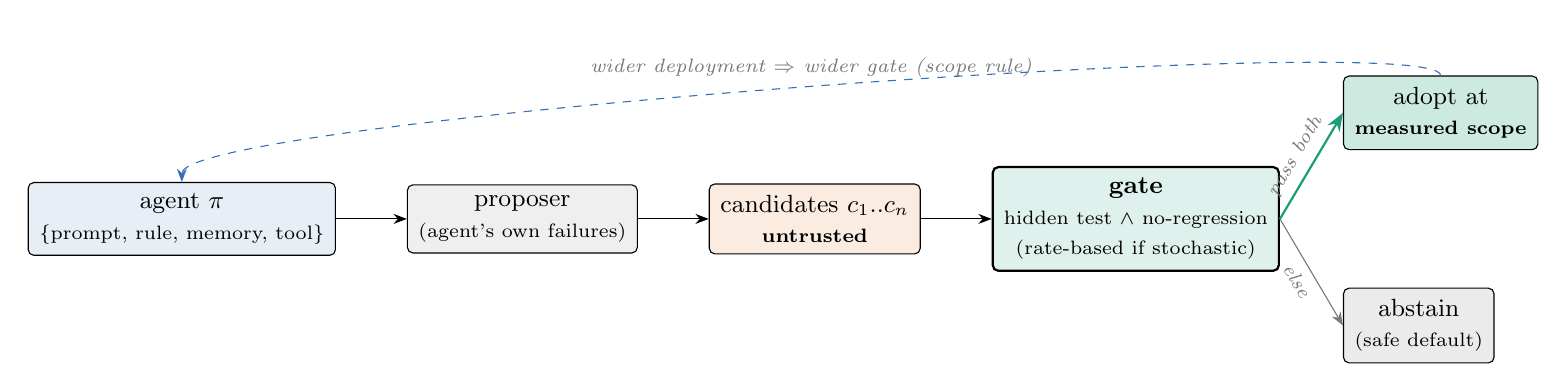
\begin{tikzpicture}[
  node distance=5mm and 9mm, font=\small,
  box/.style={draw, rounded corners=2pt, align=center, inner sep=4pt, minimum height=8mm},
  lab/.style={font=\scriptsize\itshape, text=vgray}
]
\node[box, fill=vblue!12] (agent) {agent $\pi$\\\scriptsize \{prompt, rule, memory, tool\}};
\node[box, right=of agent, fill=vgray!12] (prop) {proposer\\\scriptsize (agent's own failures)};
\node[box, right=of prop, fill=vbad!12] (cand) {candidates $c_1..c_n$\\\scriptsize \textbf{untrusted}};
\node[box, right=of cand, fill=vok!14, thick] (gate) {\textbf{gate}\\\scriptsize hidden test $\wedge$ no-regression\\\scriptsize (rate-based if stochastic)};
\node[box, above right=2mm and 8mm of gate, fill=vok!22] (adopt) {adopt at\\\scriptsize \textbf{measured scope}};
\node[box, below right=2mm and 8mm of gate, fill=vgray!15] (abst) {abstain\\\scriptsize (safe default)};
\draw[-{Stealth}] (agent) -- (prop);
\draw[-{Stealth}] (prop) -- (cand);
\draw[-{Stealth}] (cand) -- (gate);
\draw[-{Stealth}, vok, thick] (gate.east) -- (adopt.west) node[midway, above, sloped, lab] {pass both};
\draw[-{Stealth}, vgray] (gate.east) -- (abst.west) node[midway, below, sloped, lab] {else};
\draw[-{Stealth}, dashed, vblue] (adopt.north) .. controls +(0,6mm) and +(0,8mm) .. (agent.north)
  node[pos=.5, above, lab] {wider deployment $\Rightarrow$ wider gate (scope rule)};
\end{tikzpicture}%
}
\caption{The self-verifying agent. Every self-modification is untrusted until it clears a hidden
(held-out, executed where possible) test \emph{and} a regression check over the existing capability
profile; otherwise the agent abstains. A verdict is valid only at the scope it was measured---global
adoption requires a deployment-scope gate.}
\label{fig:gate}
\end{figure}

\section{Fake improvement is the norm}
\label{sec:fake}

\paragraph{Setup.} Text experiments use a 7B instruct model (Qwen2.5-7B-Instruct) as both proposer and
substrate; the judge/abstention substrate underneath was validated separately (a zero-shot reading judge
at 0.949 vs.\ a tuned guardrail's 0.789 on a sealed benchmark, with calibrated abstention transferring
to 4/6 unseen domains). Code experiments execute real Python against held-out unit tests.

\paragraph{Fine-tuning level.} Among three candidate LoRA fine-tunes of the judge, the one trained on a
single source memorizes it (train loss $0.000$, in-distribution $0.993$) and generalizes worst
(held-out $0.507$). Naive selection (best in-distribution) deploys exactly this memorizer; held-out
selection deploys the broad candidate ($0.578$).

\paragraph{Regression is silent.} Fine-tuning to fix one weak source costs another source $-0.16$ while
the target barely moves ($+0.005$); a 1-D ``did the target improve?'' check misses it entirely. A
retention-replay candidate removes the regression (worst old-capability $\Delta = 0.000$). This
reproduces, on a judge, the classic naive-correction backfire---and previews the embodied result of
\S\ref{sec:scope} in miniature.

\paragraph{Tool rewrites.} Asked to extend its own Python tool, the agent's proposal set contains a
hardcoded lookup of the observed examples in \textbf{100\% of 24 decisions}; the seen score cannot
distinguish it from the general tool (both $1.00$). Naive selection therefore ships a broken tool
\textbf{59\%} of the time. \emph{Executing} candidates on held-out inputs ships \textbf{0\%}, while
still adopting a working tool in 88\% of decisions.

\paragraph{Real code.} On MBPP ($n{=}100$) and HumanEval ($n{=}80$), a genuine overfit---a solution
passing the shown test and failing held-out tests---appears on \textbf{29\% / 30\%} of problems
respectively. Where it exists, naive ships it \textbf{19/29} and \textbf{21/24} times; the verifier
\textbf{0 on both}. Restricted to problems the agent can solve (removing the abstain-on-unsolvable
confound), naive ships a held-out-failing solution \textbf{12\% on both benchmarks}, the executing
verifier \textbf{0\%}. Two independent benchmarks, near-identical rates: the effect is a property of the
self-modification stream, not of a dataset (Figure~\ref{fig:bars}).

\begin{figure}[t]
\centering
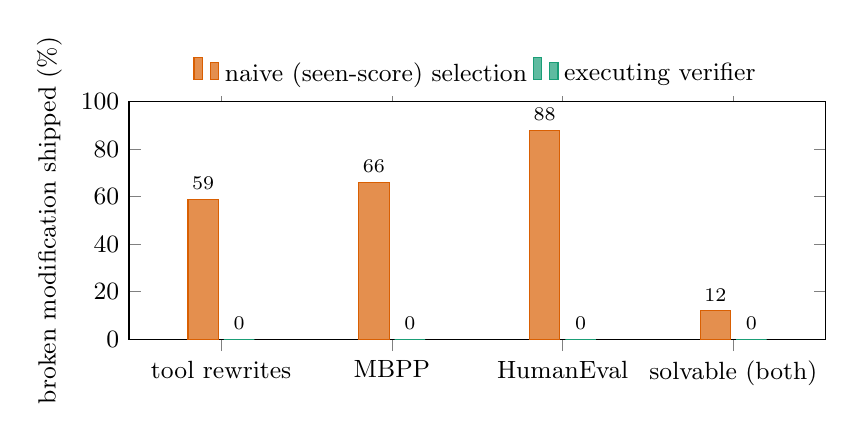
\begin{tikzpicture}
\begin{axis}[
  ybar, width=.86\linewidth, height=4.6cm,
  ylabel={\small broken modification shipped (\%)},
  symbolic x coords={tool rewrites, MBPP, HumanEval, solvable (both)},
  xtick=data, ymin=0, ymax=100,
  enlarge x limits=0.18,
  bar width=11pt,
  legend style={at={(0.5,1.02)}, anchor=south, legend columns=2, font=\small, draw=none},
  tick label style={font=\small},
  nodes near coords, every node near coord/.append style={font=\scriptsize},
]
\addplot[fill=vbad!70, draw=vbad] coordinates
  {(tool rewrites,59) (MBPP,66) (HumanEval,88) (solvable (both),12)};
\addplot[fill=vok!70, draw=vok] coordinates
  {(tool rewrites,0) (MBPP,0) (HumanEval,0) (solvable (both),0)};
\legend{naive (seen-score) selection, executing verifier}
\end{axis}
\end{tikzpicture}
\caption{The single adoption decision. When a fake modification exists, naive selection by the score on
the data the modification was derived from ships it 59--88\% of the time; the verifier (execution on
held-out data + regression check) ships 0\% across all four settings, while still adopting real
improvements (88\% of tool decisions; 68\% of MBPP problems).}
\label{fig:bars}
\end{figure}

\subsection{The flagship decision, and the autonomous loop}
\label{sec:flagship}

An agent with capability A ($1.00$) and target B ($0.00$) proposes rule-edits from its own failures. The
verifier adopts the edit that fixes B \emph{and} keeps A---\textbf{rejecting the edit that fixes B best
(hidden $1.00$) because it regresses A}---ending at $\text{A}=1.00$, $\text{B}=0.83$ (mean $0.92$) vs.\
naive $0.67$. The regression check is not decoration: the best target-fix can be the worst adoption. The
loop also closes autonomously: forced to fit patterns rather than rationalize, the proposer induces the
true hidden rule among its candidates and the verifier selects it (2/2 tasks).

\subsection{Honest negative: cumulative compounding}
\label{sec:negative}

Over 3 acquisition rounds the gated agent leads at every round ($0.88$ vs.\ $0.79$ final). At 5 rounds
the cumulative-mean advantage shrinks to $+0.03$: worst-case capability becomes dominated by
new-task acquisition noise, not by regression. The robust claim in this paper is the \emph{per-decision}
advantage; large multi-round compounding is not demonstrated on these substrates and we do not claim it.

\section{Embodied: the full arc on a real driving system}
\label{sec:embodied}

We instantiate the same gate on CARLA/Bench2Drive~\citep{dosovitskiy2017carla,jia2024bench2drive} with a
real end-to-end student (the LEAD tfv6 transfuser-family stack) and its privileged expert as teacher.
This section is one continuous, pre-registered narrative: flakiness forces a statistical gate
(\S\ref{sec:flaky}); the gate rejects a harmful fix and accepts a real one (\S\ref{sec:acceptedfix});
the accepted candidate is then \emph{globally} rejected at deployment scope (\S\ref{sec:scope}); and a
ten-recipe repair search under the fixed gate ends in a mapped frontier and an honest negative
(\S\ref{sec:search}).

\subsection{Failures are flaky; verification must be rate-based}
\label{sec:flaky}

Re-running routes with the agent, weather, and configuration unchanged: route 11755 (an
\texttt{EnterActorFlow} scenario) fails $7/12=58\%$ of runs (95\% CI $[0.32, 0.81]$)---the same route
flips PASS/FAIL run to run---while three routes labeled FAILURE by the single-run benchmark pass 100\%
on re-run: their recorded failures were one-off noise. Two consequences. (i)~Single-run failure labels,
the leaderboard standard, measure stochasticity as much as capability (run-to-run variance on these
benchmarks is documented~\citep{jia2024bench2drive}; we operationalize it into the gate rather than
re-discover it). (ii)~Verifying a fix means comparing failure \emph{rates}: confirming a
$58\%\!\to\!20\%$ improvement needs ${\sim}19$ runs per arm at 80\% power. A naive single-run check of
an unchanged model would ``confirm a fix'' with 42\% probability.

The first live fix candidate makes the point concrete: a plausible control-layer intervention
(``drive more conservatively'') \emph{raised} the observed failure rate ($50\%\!\to\!83\%$; collisions
persisted and slow driving added penalties), and the statistical gate rejected it before deployment.

\subsection{The accepted fix: the loop closes}
\label{sec:acceptedfix}

The full cycle then ran end-to-end: student fails 11755 at 58\% $\rightarrow$ the privileged expert is
stable-perfect there ($8/8$) $\rightarrow$ 359\,MB of expert demonstrations collected on the failure
scenario plus retention routes $\rightarrow$ 10-epoch fine-tune from the released checkpoint (single
RTX~5090, ${\sim}2.5$\,h) $\rightarrow$ the pre-registered gate on fresh rollouts:
\textbf{hidden test} $0/19$ failures (baseline $7/12$; exact binomial $p = 6.0\times10^{-8}$);
\textbf{regression} $0/12$ on the retention routes $\rightarrow$ \textbf{ACCEPT}. To our knowledge this
is the first pre-registered, error-controlled statistical \emph{accept} produced inside a closed
self-improvement loop on an embodied system---and the same harness had already produced the
corresponding \emph{reject} (\S\ref{sec:flaky}).

The honest scope of that verdict, stated at the time: verified \emph{same-route repair} over fresh
stochastic rollouts plus a 3-route regression set---not cross-route generalization, and not a full
regression sweep. That scope statement is not a caveat; it is the next experiment.

\subsection{The deployment gate: same candidate, opposite verdict}
\label{sec:scope}

Is the locally-accepted candidate safe to \emph{deploy}---to swap in globally? The deployment-scope
gate answers with a screen over the 169 baseline-clean routes, then interleaved candidate/baseline
confirmation runs ($4{+}4$ per flagged route) under a pre-registered rule (confirmed regression:
candidate $\ge 3/4$ failures and baseline $\le 1/4$; global reject if any confirmed regression or pooled
candidate failure significantly above baseline).

The screen flagged 19 collision routes plus a systematic soft signature (14 routes at exactly score 70
with a red-light violation and mass minimum-speed infractions---a behavioral warp, not noise). The
confirmation batch (176/176 valid interleaved runs) returned:
\textbf{12 confirmed regressions}; pooled on flagged routes, candidate $53/76 = 70\%$ vs.\ baseline
$5/76 = 7\%$ failures, one-sided $p = 8.5\times10^{-45}$ $\rightarrow$ \textbf{GLOBAL REJECT}
(Figure~\ref{fig:scope}).

The mechanism is classic catastrophic forgetting~\citep{mccloskey1989catastrophic,french1999catastrophic}:
ten epochs on ${\sim}1.6$k frames of four scenario types with a 3-route retention set warped global
driving---collisions on ordinary routes, red-light violations, slow driving everywhere. What is new here
is not the phenomenon but the demonstration: \emph{the same candidate earns a legitimate statistical
ACCEPT at target scope and a $p=8.5\times10^{-45}$ REJECT at deployment scope, on a real system, under
pre-registered rules}. Single-target evaluation---the standard practice when a fix is verified at
all---would have shipped this model. The 3-route retention check passed ($0/12$) because those routes
happen to sit among the least-affected; a narrow regression set does not just under-measure damage, it
can systematically miss it. \textbf{Verification scope must equal deployment scope.} Nothing was
adopted; the deployed capability floor never dropped.

\begin{figure}[t]
\centering
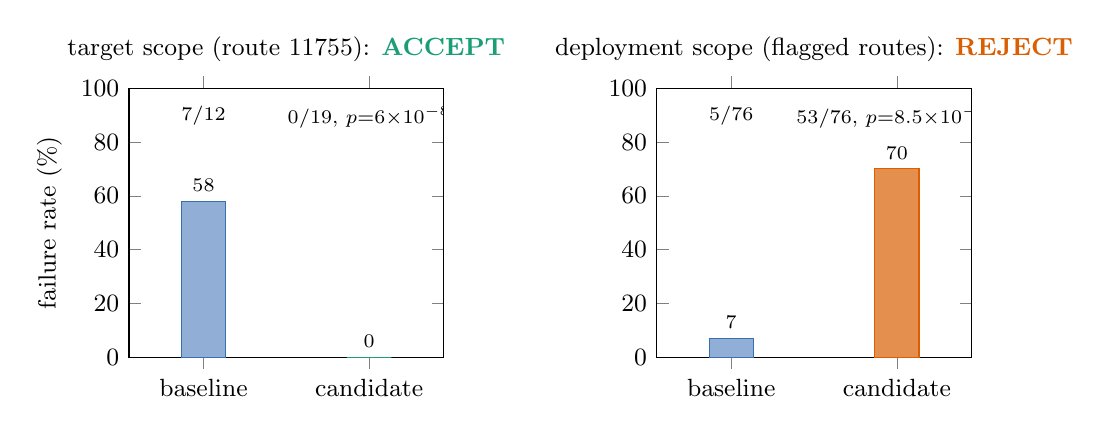
\begin{tikzpicture}
\begin{axis}[
  name=left,
  ybar, width=.46\linewidth, height=5.0cm,
  title={\small target scope (route 11755): \textcolor{vok}{\textbf{ACCEPT}}},
  ylabel={\small failure rate (\%)},
  symbolic x coords={baseline, candidate},
  xtick={baseline, candidate}, ymin=0, ymax=100, bar width=16pt,
  enlarge x limits=0.45,
  tick label style={font=\small},
  nodes near coords, every node near coord/.append style={font=\scriptsize},
]
\addplot[fill=vblue!55, draw=vblue, bar shift=0pt] coordinates {(baseline,58)};
\addplot[fill=vok!70, draw=vok, bar shift=0pt] coordinates {(candidate,0)};
\node[font=\scriptsize, anchor=north] at (axis cs:candidate,97) {$0/19$, $p{=}6{\times}10^{-8}$};
\node[font=\scriptsize, anchor=north] at (axis cs:baseline,97) {$7/12$};
\end{axis}
\begin{axis}[
  at={(left.outer east)}, anchor=outer west, xshift=4mm,
  ybar, width=.46\linewidth, height=5.0cm,
  title={\small deployment scope (flagged routes): \textcolor{vbad}{\textbf{REJECT}}},
  symbolic x coords={baseline, candidate},
  xtick={baseline, candidate}, ymin=0, ymax=100, bar width=16pt,
  enlarge x limits=0.45,
  tick label style={font=\small},
  nodes near coords, every node near coord/.append style={font=\scriptsize},
]
\addplot[fill=vblue!55, draw=vblue, bar shift=0pt] coordinates {(baseline,7)};
\addplot[fill=vbad!70, draw=vbad, bar shift=0pt] coordinates {(candidate,70)};
\node[font=\scriptsize, anchor=north] at (axis cs:candidate,97) {$53/76$, $p{=}8.5{\times}10^{-45}$};
\node[font=\scriptsize, anchor=north] at (axis cs:baseline,97) {$5/76$};
\end{axis}
\end{tikzpicture}
\caption{One candidate, two scopes, opposite verdicts---both correct at their scope. Left: the fine-tune
genuinely repairs its target route ($58\%\!\to\!0\%$ over 19 fresh rollouts). Right: the same model at
deployment scope collides on ordinary routes the baseline drives cleanly (12 confirmed regressions;
pooled $70\%$ vs.\ $7\%$). Single-target evaluation would have shipped it.}
\label{fig:scope}
\end{figure}

\subsection{The ten-recipe repair search: a mapped frontier, an honest negative, a gate that held}
\label{sec:search}

Can a better fine-tuning recipe pass \emph{both} gates? We ran a pre-registered, timeboxed search: the
gate stays fixed; only the recipe iterates. Local panel (pre-registered lines): fix arm 11755
$\le 2/8$ failures; retention arm over the 12 previously-confirmed regression routes, pooled
$\le 30\%$; deployment gate as in \S\ref{sec:scope} for any panel-passer. Ten recipes were evaluated
in total (Table~\ref{tab:ledger}; ${\sim}450$ verification rollouts): the control-layer intervention,
the original narrow fine-tune, and eight variants spanning training length, retention breadth, mixture
ratios (via the stack's native two-bucket oversampling), fix-family breadth, targeted retention
collection, and backbone freezing (head-only, $16.6$M trainable parameters).

\begin{table}[t]
\caption{The repair-search ledger. Every verdict pre-registered; the gate never adopted a regression.
Fix line: $\le 2/8$ failures on route 11755. Retention line: $\le 30\%$ pooled failures on the 12
confirmed-regression routes. $^{\dagger}$K1's retention was measured at deployment scope
(\S\ref{sec:scope}); panel lines were pre-registered after it.}
\label{tab:ledger}
\centering
\footnotesize
\setlength{\tabcolsep}{4.5pt}
\begin{tabular}{@{}lllll@{}}
\toprule
\# & recipe (one variable at a time where possible) & fix 11755 & retention & verdict \\
\midrule
0 & control-layer ``drive conservatively'' (no training) & worse ($50{\to}83\%$) & --- & REJECT \\
K1 & narrow data, 10 epochs, full FT & $0/19$ \checkmark & 12 confirmed reg.$^{\dagger}$ & \textbf{global REJECT} \\
K2a & K1 data, 3 epochs & $0/8$ \checkmark & $12/12$ routes fail & REJECT \\
K2b & broad retention (17 routes), 3 ep & $4/8$ & $33\%$ & REJECT (fix diluted) \\
A1 & fix $40\%$ oversample, 3 ep & $4/8$ & $25\%$ \checkmark & REJECT (fix diluted) \\
A2 & fix $60\%$ oversample, 5 ep & $0/8$ \checkmark & $29\%$ \checkmark & \textbf{panel PASS} $\to$ \\
  & \quad$\hookrightarrow$ deployment gate & --- & 6 confirmed reg., $p{=}2.5{\times}10^{-20}$ & \textbf{global REJECT} \\
A3 & A2 + fix-family demos in fix bucket & $6/7$ & (cut short) & REJECT (family conflict) \\
A4 & A2 fix bucket + targeted retention & $4/8$ & $33\%$ & REJECT \\
A5 & A4 + frozen backbone (head-only) & $4/8$ & ${\sim}31\%$ & REJECT \\
A6 & A2 data + frozen backbone & $3/8$ & $\mathbf{17\%}$ \checkmark & REJECT (fix, by one run) \\
\bottomrule
\end{tabular}
\end{table}

\begin{figure}[t]
\centering
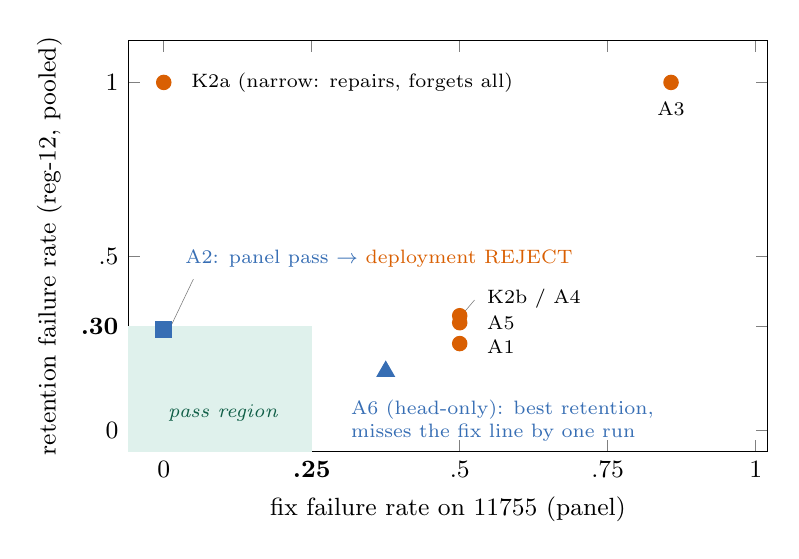
\begin{tikzpicture}
\begin{axis}[
  width=.8\linewidth, height=6.8cm,
  xlabel={\small fix failure rate on 11755 (panel)},
  ylabel={\small retention failure rate (reg-12, pooled)},
  xmin=-0.06, xmax=1.02, ymin=-0.06, ymax=1.12,
  xtick={0,.25,.5,.75,1}, ytick={0,.3,.5,1},
  xticklabels={0,\textbf{.25},.5,.75,1}, yticklabels={0,\textbf{.30},.5,1},
  tick label style={font=\small},
  grid=none,
]
\fill[vok!14] (axis cs:-0.06,-0.06) rectangle (axis cs:0.25,0.30);
\node[font=\scriptsize\itshape, text=vok!60!black] at (axis cs:0.10,0.05) {pass region};
\addplot[only marks, mark=*, mark size=2.6pt, color=vbad] coordinates {
  (0.0,1.0) (0.5,0.33) (0.5,0.25) (0.857,1.0) (0.5,0.31)
};
\addplot[only marks, mark=square*, mark size=2.8pt, color=vblue] coordinates {(0.0,0.29)};
\addplot[only marks, mark=triangle*, mark size=3.6pt, color=vblue] coordinates {(0.375,0.17)};
\node[font=\scriptsize, anchor=west] at (axis cs:0.03,1.0) {K2a (narrow: repairs, forgets all)};
\node[font=\scriptsize, anchor=north] at (axis cs:0.857,0.97) {A3};
\node[font=\scriptsize, anchor=west] at (axis cs:0.53,0.38) {K2b / A4};
\node[font=\scriptsize, anchor=west] at (axis cs:0.53,0.31) {A5};
\node[font=\scriptsize, anchor=west] at (axis cs:0.53,0.24) {A1};
\draw[vgray, very thin] (axis cs:0.505,0.335) -- (axis cs:0.525,0.375);
\node[font=\scriptsize, anchor=south west, text=vblue] at (axis cs:0.02,0.44)
  {A2: panel pass $\to$ \textcolor{vbad}{deployment REJECT}};
\draw[vgray, very thin] (axis cs:0.012,0.30) -- (axis cs:0.05,0.435);
\node[font=\scriptsize, align=left, anchor=north west, text=vblue] at (axis cs:0.30,0.115)
  {A6 (head-only): best retention,\\misses the fix line by one run};
\end{axis}
\end{tikzpicture}
\caption{The measured repair--retention frontier across the recipe search (panel scope; A3's retention
arm was cut short and is plotted at its decided axis only). Narrow full fine-tuning repairs and forgets
(upper left); breadth or head-only training retains and dilutes (lower right). A2 enters the pass region
at panel scope and is then rejected by the deployment gate---the scope rule again. No recipe passes both
gates at this budget.}
\label{fig:frontier}
\end{figure}

The search converged, honestly, to a mapped trade-off rather than a winner (Figure~\ref{fig:frontier}).
Its findings:

\begin{itemize}
\item \textbf{Forgetting here is a data-breadth problem, not a training-length problem}: cutting epochs
$10\!\to\!3$ on narrow data preserved the repair and all twelve regressions.
\item \textbf{The stability--plasticity see-saw is real and sits in the planning head}: with fix data
identical to the panel-passing recipe, merely \emph{adding} retention data broke the repair (A4);
freezing the perception backbone did not recover it (A5); the interference lives in the shared planning
parameters, echoing at system scale the classic trade-off~\citep{french1999catastrophic}.
\item \textbf{Dilution is fractal}: adding same-family demonstrations to the fix bucket did not
generalize the repair---it diluted and conflicted with it one level down (A3: the family-scenario route
itself had failed $4/4$ under A2, a within-family overfit; fixing that broke 11755).
\item \textbf{Panel pass $\ne$ deployment pass, again}: A2, the one panel-passer, was rejected by the
deployment gate (6 confirmed regressions, $p=2.5\times10^{-20}$)---though the search was converging
(12 confirmed regressions $\to$ 6, global behavioral warp eliminated).
\item \textbf{Bounded negative}: at this budget (a single consumer GPU, the stack's native fine-tuning
machinery, ${\sim}450$ verification rollouts), no recipe passed both gates. Full fine-tuning repairs
perfectly and collapses globally; head-only training retains best ($17\%$) and misses the fix line by
one run ($3/8$). We report this as a first-class result, not a failure of the method under test: the
method under test is the \emph{gate}, and the gate did exactly its job.
\end{itemize}

Through the entire search---ten recipes, every verdict pre-registered---\textbf{zero regressions were
adopted and the deployed capability floor never dropped}. The gate demonstrated all four of its decision
modes on a real system: accept-real (\S\ref{sec:acceptedfix}), reject-harmful (\S\ref{sec:flaky},
\S\ref{sec:scope}), reject-insufficient (A6), and protect-through-search (this section). A
pre-registered caution for practitioners: iterating recipes against a fixed screen risks overfitting the
gate itself (the embodied form of the gate-reuse effect of \S\ref{sec:method}); any finally-accepted
candidate must additionally pass held-back validation never used during iteration.

\subsection{The outer loop, automated}
\label{sec:automated}

The searches above were orchestrated by a human (verdicts were always computed by the gate). A fair
objection: is this a self-improvement \emph{loop}, or a human-curated search? We answer by removing the
human. Under a pre-registered protocol (win conditions, a hard cutoff, and a compute fallback, all
sealed before any code was written), we implemented the outer loop as code: an \emph{append-only trial
registry} (thresholds stored at registration time, before data; trials frozen once a verdict is
computed; verdicts computed from raw counts, never stored by fiat) and a \emph{rule-based prescriber}
(the continual-learning ladder: cheapest variable $\to$ replay breadth $\to$ replay weighting $\to$
targeted replay $\to$ parameter isolation) that may only propose---the gate remains the sole adoption
authority.

\textbf{Replay (consistency).} Replaying the S1 search through this machinery reproduces all 12
recorded verdicts exactly from raw counts---including the scope splits and the honest early-stops---and
the prescriber emits the move the human search actually made at 9/9 recipe transitions, both scope
escalations, and the budget-exhausted closure. Sealed caveat: the rules were distilled \emph{from} that
search, so replay validates the distillation, not generality.

\textbf{New trials (zero human verdicts).} The automated loop then ran fresh trials end-to-end (the
human launched a script and read the result). On 100 never-before-used MBPP problems, with each
problem's tests split visible / gate-hidden / \emph{audit} (the gate never sees the audit; without this
split ``the gate ships zero failures'' would be true by construction): naive ships an audit-failing
solution $41/100$; the gate adopts 59, abstains 41, and its adoptions fail audit $5/59 = 8.5\%$---a
registry-computed \textbf{ACCEPT} ($p = 2.8\times10^{-8}$). Note the honest non-zero: the audit
measures what the gate buys ($41\%\!\to\!8.5\%$), not a tautology. The prescriber---not a
human---then ordered scope escalation, and on the remaining 26 fresh HumanEval problems naive shipped
\emph{zero} audit failures: the registry returned \textbf{REJECT} (no improvement evidence, $p=1$),
declining to manufacture significance where none exists, and the prescriber, hitting a state its rules
do not map, handed back to the operator and stopped rather than guessing. One accept, one honest null,
no human in the verdict path: the title's claim is literal for these trials.

\section{What is and is not established}
\label{sec:established}

\textbf{Established.} (1)~The agent's own modification stream is adversarial by default---overfits and
lookup-hacks are pervasive across surfaces and domains, including real code. (2)~Seen/derivation-set
score carries no signal against them; held-out (on code, \emph{executed}) evaluation does. (3)~The
two-gate verifier converts this into a reliable per-decision win: $59\%\!\to\!0\%$, $19/29\!\to\!0$,
$21/24\!\to\!0$. (4)~Regression checking is necessary: the best target-fix can be the worst adoption.
(5)~In stochastic embodied domains, only rate-based statistical verification is meaningful, and it
supports both accept ($p=6\times10^{-8}$) and reject ($p=8.5\times10^{-45}$) with error control.
(6)~A verdict is only valid at its measured scope; scope-mismatched acceptance ships catastrophic
forgetting on a real system. (7)~The outer loop needs no human: registry + prescriber + gate replays
the recorded search exactly from raw counts and runs fresh trials end-to-end, accepting where evidence
exists and returning an honest null where it does not (\S\ref{sec:automated}).

\textbf{Not established.} Large cumulative multi-round gains (\S\ref{sec:negative}); verified
self-improvement on hard tasks where no candidate transfers (the verifier then correctly adopts
nothing---safe, but not improvement); a deployment-gate-passing embodied repair (\S\ref{sec:search}:
bounded negative at this budget); behavior beyond a 7B proposer, benchmark-scale substrates, one vehicle
stack, and one simulator.

\section{Related work and claim boundaries}
\label{sec:related}

\textbf{Self-improving agents} (Reflexion~\citep{shinn2023reflexion}; ExpeL~\citep{zhao2024expel};
AutoGuide~\citep{fu2024autoguide}; Voyager~\citep{wang2023voyager}) supply the proposer we gate.
\textbf{That self-generated improvement is frequently fake is established}: agent benchmarks are
reward-hackable~\citep{rdi2026hacking}; frontier agents hack their evaluations
spontaneously~\citep{metr2025rewardhacking}; a self-modifying system falsified its own
metric~\citep{zhang2025dgm}; self-reflection confabulates. \textbf{Gating self-modification is an
emerging thread}: PACE shows that greedy ``keep it if the score went up'' acceptance is uncontrolled
adaptive multiple testing and replaces it with anytime-valid (e-process) commit tests on text-agent
loops~\citep{pace2026}---the same diagnosis as ours, in the statistical dimension we
pre-register; GRASP gates skill-library edits on probe-based net improvement~\citep{grasp2026}; GRACE
uses an update-rejection gate inside prompt optimization~\citep{grace2025}; and sequential statistics
have been brought to robot policy comparison as an offline evaluation tool~\citep{beyondbinary2025}.
None of these operate on an embodied system inside the loop, and none demonstrate the
deployment-scope failure. \textbf{Driving-benchmark noise is
documented}~\citep{jia2024bench2drive,dosovitskiy2017carla}, with published scores typically
single-run. \textbf{Continual learning} names our regression phenomenon catastrophic
forgetting~\citep{mccloskey1989catastrophic,french1999catastrophic,kirkpatrick2017ewc}, and our repair
recipes (replay ratios, freezing, DAgger-style collection~\citep{ross2011dagger,hu2022lora}) are its
textbook tools deliberately reused, not claimed as new.

We therefore \emph{do not} claim: the first observation that self-improvement is often fake; the first
statistical gate for self-improving agents; or the discovery of driving-benchmark flakiness. To our
knowledge, what \emph{is} unclaimed before this work: (a)~fake-improvement \emph{rates measured across
all four modification surfaces} under one protocol, plus two real code benchmarks; (b)~a
\emph{pre-registered, error-controlled statistical accept and reject operating inside a closed
self-improvement loop on an embodied system}, including the operationalization of run-to-run noise into
a failure-rate gate; and (c)~the \emph{deployment-scope demonstration}---a narrowly-scoped gate accepts
a change whose collateral damage a scope-matched gate then catches, on a real system, followed by a
gate-protected recipe search ending in a mapped frontier. (Literature scan of July 2026; the space moves
fast.)

\section{Limitations}
\label{sec:limits}

A 7B proposer; controlled/benchmark substrates; six-item held-out sets on the toy loops (granularity
$0.17$); one vehicle stack and one simulator; the embodied fix targets one (representative, flakiest)
failure route with an 8-run fix arm and 24-run retention arm at panel scope---adequate for the
pre-registered lines, underpowered for small effects; the bounded negative of \S\ref{sec:search} is a
statement about this training budget and recipe family (parameter-efficient adapters and larger fix-side
data remain untested). Gate reuse must be budgeted (\S\ref{sec:method}); we spec but do not automate it.
Multi-round compounding may appear on richer substrates; we did not demonstrate it.

\section{Conclusion}

Across text, real code, and embodied driving, self-improvement without verification ships fakes at
rates of 12--88\%, and the fakes are supplied by the loop itself. A verifier that demands held-out
transfer and no regression---nothing more exotic---reduced shipped fakes to zero in our experiments
while still adopting real improvements; its statistical form both accepted a real embodied repair and
rejected the same candidate at deployment scope before it could ship catastrophic forgetting; and under
a ten-recipe search it held the capability floor while honestly reporting that no recipe earned
adoption. If self-improving agents are to be trusted with their own modification stream, the verifier
is not a component of the loop. \textbf{The verifier \emph{is} the loop; the rest is a proposal
generator.}

\begin{ack}
Removed for anonymous review.
\end{ack}

\bibliographystyle{plainnat}
\bibliography{references}

\appendix

\section{Reproducibility}
All numbers in this paper are produced by scripts in the accompanying repository (anonymized for
review); each result entry in the repository's ledger names the script and exact configuration that
produced it. Text and code experiments run on a single GPU with a 7B open-weight model; embodied
experiments use CARLA 0.9.15 + Bench2Drive with the LEAD stack on a single RTX~5090 (Windows-native).
The gate itself is released as a dependency-free library (\texttt{vsi\_gate.py}) exposing
\texttt{gate()} (score form) and \texttt{gate\_rate()} (exact-binomial failure-rate form), with a
deterministic no-LLM demo.

\section{Pre-registered decision rules (embodied)}
\label{app:prereg}
Fixed before the corresponding runs, unchanged throughout: \textbf{(local panel)} fix arm: route 11755,
8 fresh rollouts, pass iff $\le 2$ failures; retention arm: the 12 confirmed-regression routes
$\times 2$, pass iff pooled failures $\le 30\%$; both required. \textbf{(deployment gate)} screen all
169 baseline-clean routes once; flag any failure; triage pure-artifact flags (minimum-speed/lane-only)
out; confirm each flagged route with interleaved candidate/baseline runs ($4{+}4$); confirmed regression
iff candidate $\ge 3/4$ failures and baseline $\le 1/4$; global REJECT iff $\ge 1$ confirmed regression
or pooled candidate failure significantly above baseline (one-sided exact test, $\alpha=0.05$).
\textbf{(rate gate)} a fix claim requires a one-sided exact-binomial significant reduction against the
measured baseline rate, power-planned before collection (e.g.\ $58\%\!\to\!20\%$ requires
${\sim}19$ runs/arm at $80\%$ power).

\end{document}
